\section{Texture Advection}
Motivation: \emph{Dense} visualisation of vector fields without any seed points.

\begin{description}
\item Methods for \emph{static} fields:
    
    LIC - Line integral convolution (Cabral/Leedom 1993)
\item Methods for \emph{time-dependent} fields:
    \begin{itemize}
        \item LEA - Lagrangian-Eulerian Advection (Jobard et al. 2001)
        \item IBFV - Image-Based Flow VIs (van Wijk 2002)
    \end{itemize}
\item Methods for vector fields \emph{on surfaces}
    \begin{itemize}
        \item IBFVS - IBV for Surfaces
        \item ISA - Image-Space Advection (Laramee 2003)
    \end{itemize}

\end{description}

\subsection{Line Integral Convolution}
Line integral convolution (LIC) is a family of 10+ variants. The original method by Cabral and Leedom assumes 2D vector fields on rectilinear grids.

Basic idea:
\begin{enumerate}
    \item Generate a grey level image of random pixels at the desired resolution.
    \item Compute forward and backward streamline segments of fixed arc length for all pixels.
    \item Sample the random image along the streamline and compute the average (i.e. convolve with a box filter).
    \item Use the computed values as the pixels of the output image.
    \item Stretch the range of the output image.
\end{enumerate}

LIC images can be combined with a colour coding of a scalar field:
\begin{description}
\item in \emph{HSV} space:
    \begin{description}
        \item hue: Scalar field
        \item saturation: 1
        \item value: LIC
    \end{description}
\item in \emph{HLS} space:
    \begin{description}
        \item hue: scalar field
        \item lightness: LIC
        \item saturation: 1
    \end{description}
\end{description}

\paragraph{The Fast LIC method} (Stalling) is an order of magnitude faster by reusing parts of streamlines where possible. Fast LIC is the basis of most the newer LIC methods.

\paragraph{LIC for unstructured grids} (Battke) uses a \emph{procedural} 3D random image. For each triangle a LIC image is computed separately and displayed as a separate texture map.

This method can also be used for \emph{vector fields on surfaces}.

\paragraph{LIC method for curvilinear grids} (Forsell). Generate a LIC in computational space $\mathcal C$ and use it as a texture map for the grid in physical space $\mathcal P$.

Problems of this approach: If parameters lines are not smooth and cell sizes have a large variation the then resulting image might show artefacts.

\paragraph{Animated LIC} The LIC of static vector fields can be easily animated to show the relative velocity magnitueds:
\begin{itemize}
    \item Use samples at constant \emph{time steps}
    \item Replace the box filter by \emph{sinusodial} filter with exactly one period.
    \item Shift the kernel \emph{backward} in steps of one sample.
\end{itemize}
This results in the texture moving forward.

\paragraph{3D LIC} LIC can be computed easily in 3D but the result is a 3D image. Rendering options:
\begin{description}
    \item Isosurfaces: NO
        
        Sensitive to noise, LIC is a near worst case!
        
    \item Direct volume rendering: Yes
\end{description}

\subsection{Multi-Layer Flow Textures}

Multi-Layer LIC-like textures (Carnecky 2012) require:
\begin{itemize}
    \item Multi-Layer screen-space data structure ("illustration buffer")
    \item Procedural 3D noise texture with constant screen-space frequency
    \item Anisotropic diffusion to obtain flow aligned texture. 
\end{itemize}

\subsection{Lagrangian-Eulerian Advection}
Dynamic behaviour can be expressed in either Eulerian or Lagrangian formulation:
\begin{description}
\item[Eulerian] or \emph{grid-based}:

Fields are given at grid nodes
\item[Lagrangian] or \emph{particle-based}: 

A set of particles is advected by the velocity field $v(x,t)$, other fields are given at particle positions.
\end{description}

The temporal change of a function $f(x,t($ \emph{while following a particle} is expressed by the \emph{material derivative} (or convective derivative):
\begin{align*}
    {Df(x,t)\over Dt} = {\delta f(x,t)\over \delta t} + \Delta f(x,t)\cdot v(x,t)
\end{align*}


\subsubsection{Lagrangian-Eulerian Advection for Vector Field Visualisation}
The LEA method for vector field visualisation (Jobard 2011) uses \emph{one particle per cell}:

Initialise a white noise texture (same as for LIC).
\begin{description}
\item For each time step do:
    \begin{description}
        \item For each particle do:
            \begin{itemize}
                \item Integrate \emph{backward} pathline segment giving a new \emph{texel value} for the cell.
                \item Integrate \emph{forward} pathline segemtn giving the new \emph{particle position} in the same cell (local coordinates modulo 1).
            \end{itemize}

    \end{description}
\end{description}
Why backward integration? The texture advection can be done as \emph{forward mapping} (Lagrangian scheme) or \emph{backward mapping} (Eulerian scheme).

With backward mapping being the better choice.

\begin{figure}[H]
    \centering
    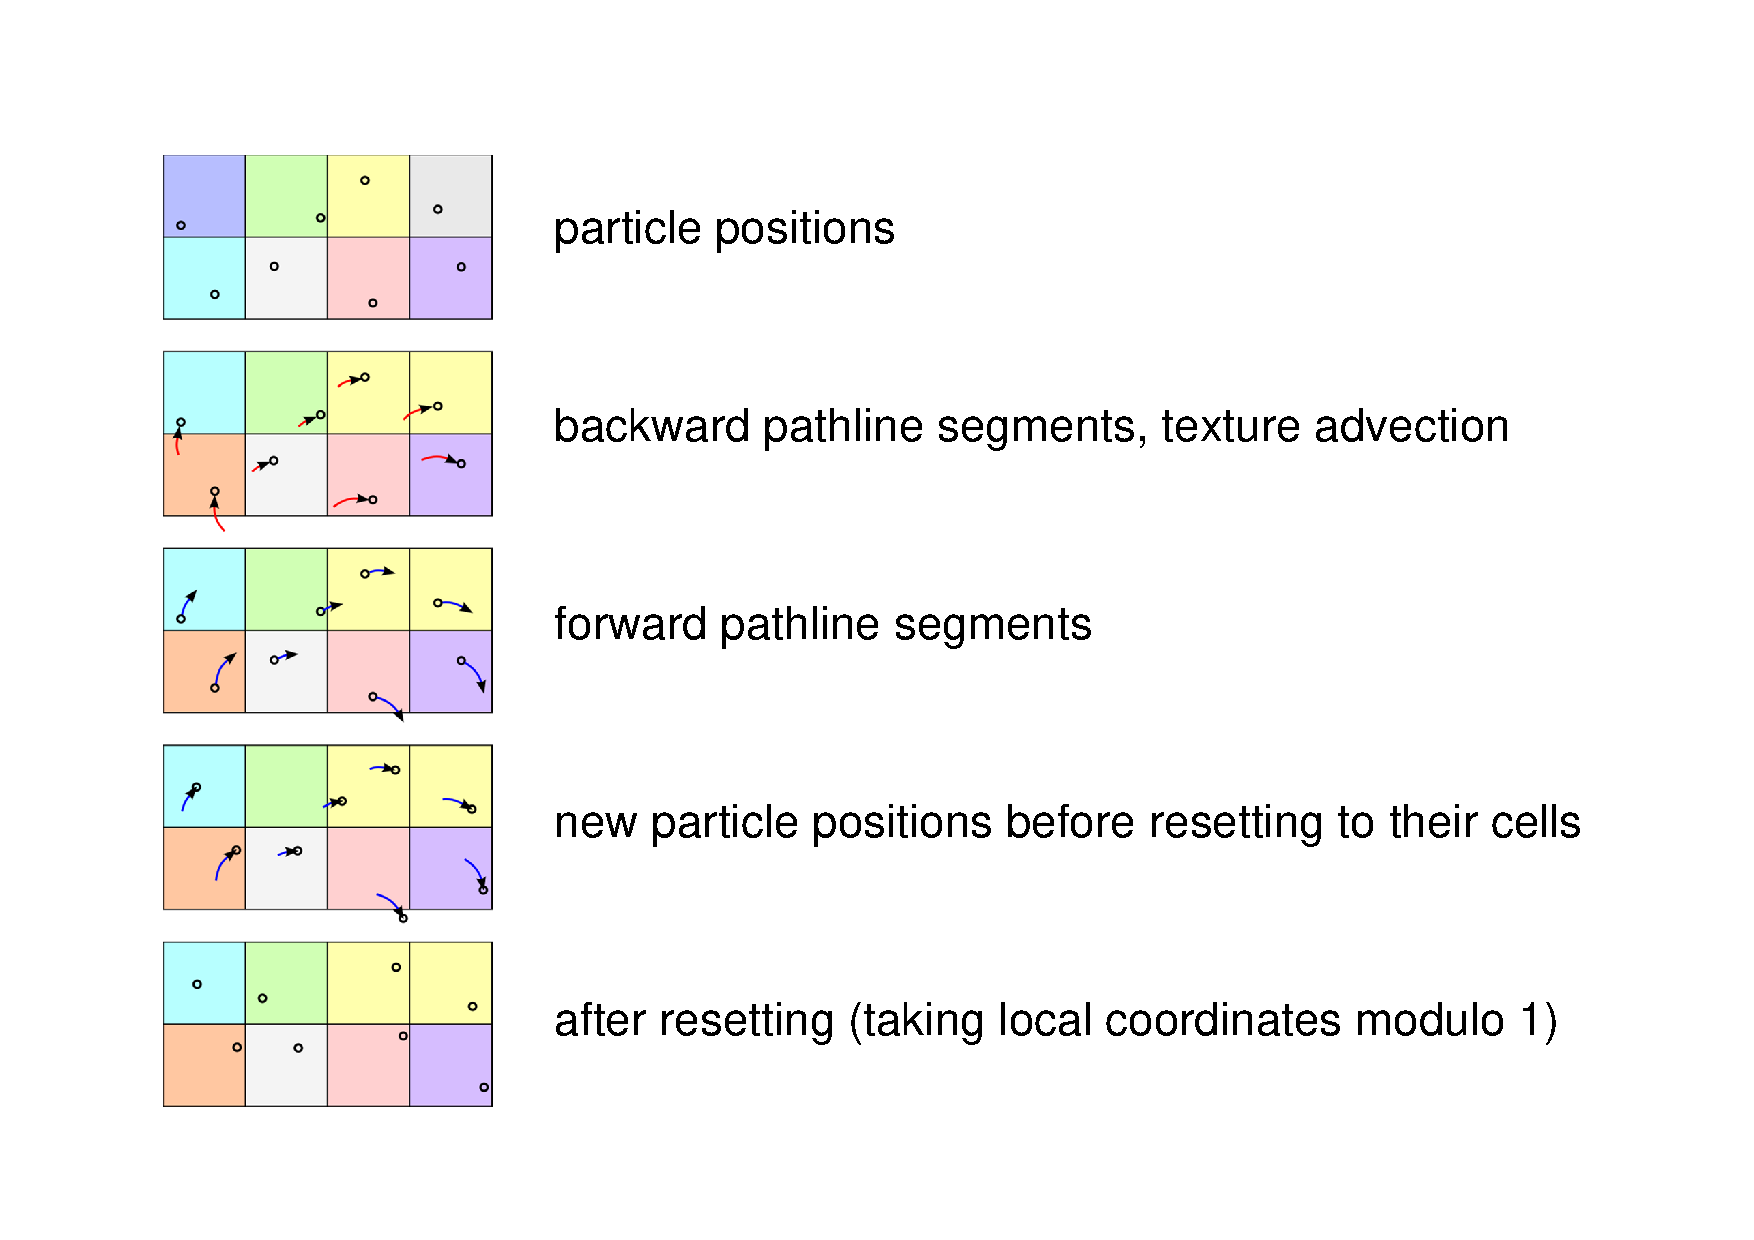
\includegraphics[width=0.8\textwidth]{img/06_eulerian_advection}
\end{figure}

\paragraph{Special choices made by LEA} $\ $ 
\begin{itemize}
    \item $1^{st}$ order integration
    \item Simplification: Forward segment = $-$backward segment
    
        Better: Backward segment = $-$previous forward semgent
    \item Add buffer cells at grid boundaries:
        \begin{itemize}
            \item Contain texture but no particles
            \item Allow texture advection at inflow boundaries
            \item Random texture is refreshed after each time step to avoid artefacts
        \end{itemize}
    \item Post-Processing: Apply a LIC filter to each image before outputting.
\end{itemize}
\paragraph{Interpolation}
Backward mapping scheme allows $2$ interpolation choices:
\begin{itemize}
    \item \emph{nearest-neighbour}
    \item Bilinear
\end{itemize}
LEA uses \emph{both}:
\begin{itemize}
    \item Nearest-neighbour is used for updating the \emph{stored} texture.
    \item Bilinear interpolation is used for \emph{displayed} texture
\end{itemize}

\paragraph{Noise injection} Backward mapping can have a duplication effect. Causes are:
\begin{itemize}
    \item Divergence of the vector field.
    \item Nearest-neighbour interpolation
\end{itemize}
\begin{figure}[H]
    \centering
    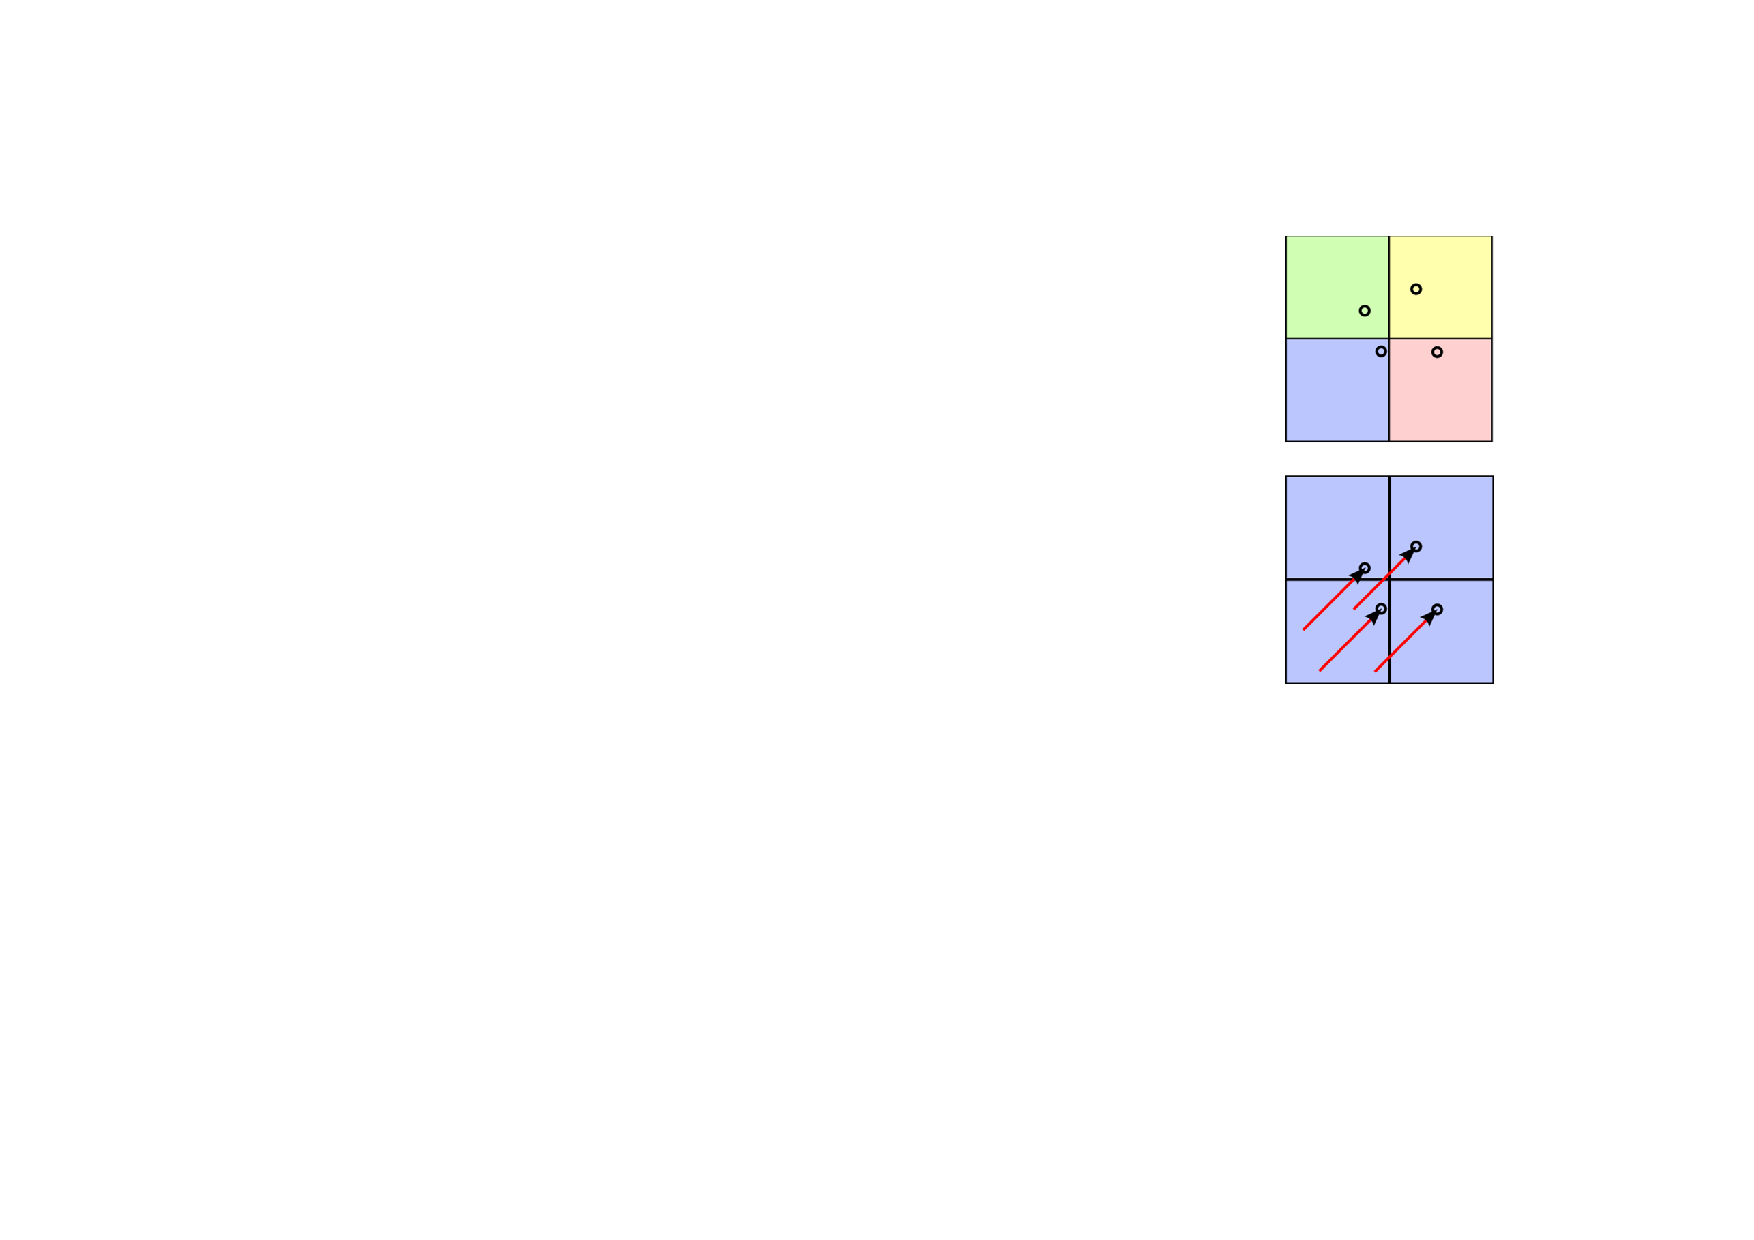
\includegraphics[width=0.4\textwidth]{img/06_noise_injection}
\end{figure}


Solution: \emph{Noise injection}: A small percentage of noise is added after each step. 

Trade-off: Keep high frequencies, but also temporal correlation.

\subsection{Image-Based Flow Visualisation}
IBFV algorithm (van Wijk 2002). Main idea:
\begin{itemize}
    \item Initialise a noise texture image.
    \item For each time step do:
        \begin{itemize}
            \item \emph{Advect nodes} of the texture image resulting in a warped grid.
            \item \emph{Render} the \emph{warped grid}, texture mapped.
            \item Resample the image to original mesh: 
            
                \emph{Read back} the rendered image to texture memory.
            \item Use as next texture image. 
        \end{itemize}
\end{itemize}
\begin{figure}[H]
    \centering
    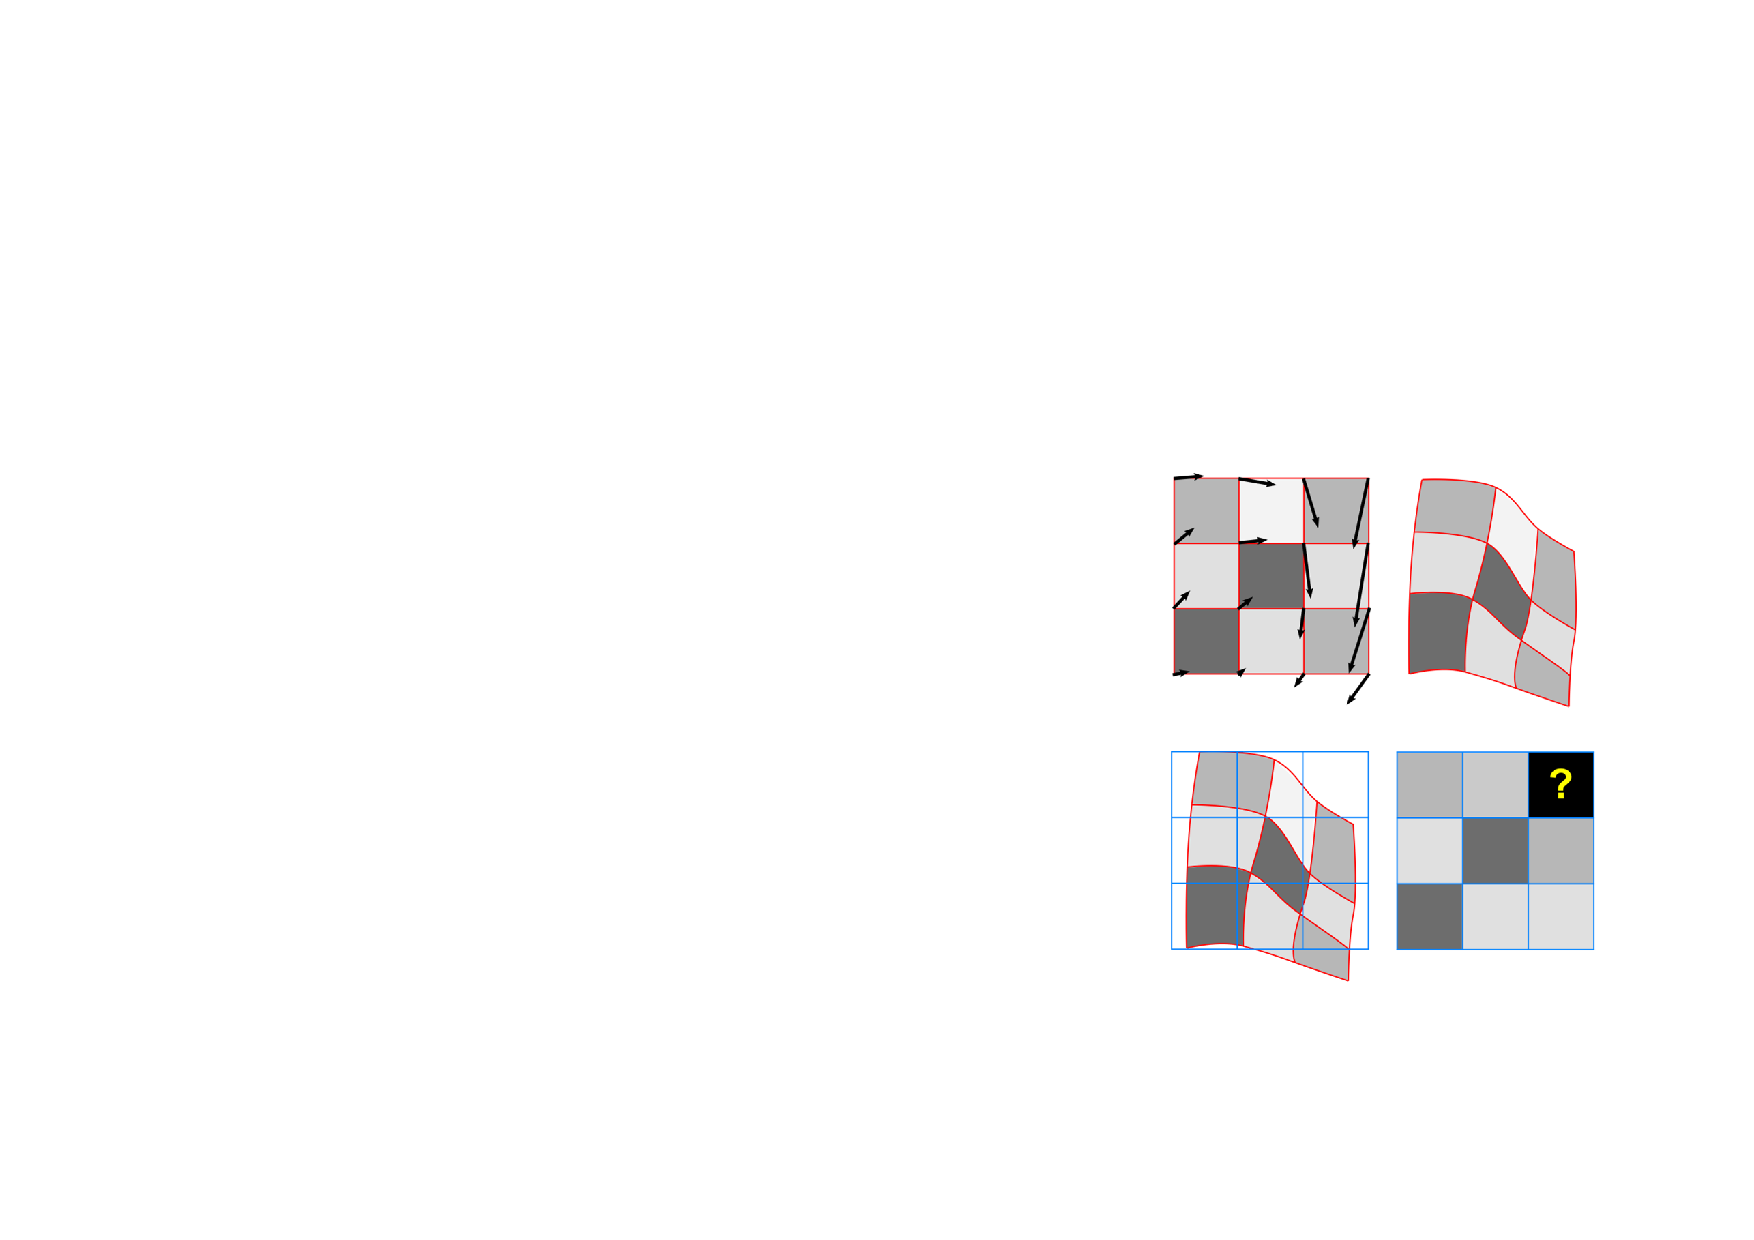
\includegraphics[width=0.4\textwidth]{img/06_ibfv}
\end{figure}


Detailed algorithm:
\begin{itemize}
    \item Initialise a noise texture image.
    \item For each time step do:
        \begin{itemize}
            \item Advect nodes of the texture image, resulting in a warped grid.
            \item Render the warped grid, texture mapped.
            \item \emph{Blend with noise image}.
            \item \emph{Apply dye injection}.
            \item Resample image to original mesh.
            \item Use as next texture image
            \item \emph{Draw overlaid graphics}
        \end{itemize}
\end{itemize}

\paragraph{Noise image}$\ $
\begin{description}
    \item \emph{Static} results in static image for steady flow
    \item \emph{Temporally coherent}, using \emph{spot noise} texture.
\end{description}

\paragraph{Boundary areas} For the boundary areas a special solution is needed. Simple solution: Don't clear the screen before redrawing. 

\paragraph{Comparison with LEA} IBFV is a much faster algorithm than LEA. The coherence is not as good.

\subsection{Texture advection in surfaces}
Texture advection on surfaces can be used for:
\begin{itemize}
    \item Boundary flow (wall shear stress)
    \item Flow on streamsurfaces
    \item Less meaningful: Project flow on other surfaces (isosurfaces)
\end{itemize}

Possible but expensive:
\begin{itemize}
    \item Work in object space
    \item Use 3D texture
\end{itemize}

Alternatives:
\begin{itemize}
    \item Work in image space:
        \begin{itemize}
            \item IBFV for surfaces (van Wijk)
            \item Image-space advection (Laramee)
        \end{itemize}
\end{itemize}

\subsection{IBFV for Surfaces}
Idea for IBFVS:
\begin{itemize}
    \item Use screen coordinates from previous rendering as texture coordinates.
    \item Advect in object space.
    
    I.e. Distort the surface mesh.
    \item Render the distorted mesh, keeping the texture coordinates
    \item Apply noise injection and blending
    \item Overlay the image
\end{itemize}

\subsection{Image-Space Advection}
Idea for ISA:
\begin{itemize}
    \item Project the velocity field to image space.
    \item Do IBFV within boundary silhouette.
    
    I.e. Advect rectangles.
    
    \item Apply noise injection and blending.
    \item Overlay image.
\end{itemize}

Comparison with IBFVS:
\begin{description}
\item Advantages:
    \begin{itemize}
        \item Projected velocity field simplifies advection
        \item No computation time is spent for hidden polygons and polygons smaller than a pixel
    \end{itemize}
\item Problems:
    \begin{itemize}
        \item Artificial continuity across interior silhouettes:
        
        ISA uses edge detection (depth discontinuities)
        
        \item The texture is not attached to the surface when the camera is moving.
    \end{itemize}

\end{description}

































